\section{Link Model}\label{sec:linkmodel}
In this section, our own Linkmodel will be described.

\subsection{Computing path loss}
To facilitate to the problems discussed in \autoref{sec:reachi-experiments}, we have devised our own linkmodel to compute path loss. Our model computes path loss based on the distance of the link and the percentage of that distance that is in a building. Building and other obstructions in the environment cause more severe path loss, and as such should be considered to punish the signal more. Our model limits to only buildings. The idea is to generate a map of the area that the nodes are located in as an image, then when computing the path loss of a link, look up the colour of all pixels in a straight line between the nodes  of link and count how many is a building. This gives a percentage for how much of the distance is covered by buildings. An pseudo code implementation of the computation can be seen on \autoref{algo:linkmodel:compute-building-percentage}.

\begin{algorithm}[H]
    \DontPrintSemicolon
    \SetKwFunction{FLoSModelCompute}{ComputeBuildingPercentage}
    \SetKwProg{Fn}{Function}{}{}

    \Fn{\FLoSModelCompute{$l$}}{
        $(n_1,\ n_2) \leftarrow \mathit{nodes}(l)$\;
        $(x_1,\ y_1) \leftarrow$ compute position for $n_1$\;
        $(x_2,\ y_2) \leftarrow$ compute position for $n_2$\;
        \;
        $\mathit{pixels} \leftarrow 0$\;
        $\mathit{buildings} \leftarrow 0$\;
        \While{$\lambda \in \{0 \dots 1\}$}{
            $(x,\ y) \leftarrow \lambda \cdot (x_1,\ y_1) + (1 - \lambda)\cdot(x_2,y_2)$\;
            \If{position ($x$, $y$) is a building}{
                $\mathit{buildings} \leftarrow \mathit{buildings} + 1$\;
            }
            $\mathit{pixels} \leftarrow \mathit{pixels} + 1$\;
        }

        \KwRet $\mathit{buildings} / \mathit{pixels}$\;
    }
    \caption{The ComputeBuildingPercentage function.}
    \label{algo:linkmodel:compute-building-percentage}
\end{algorithm}


We define two functions, $\mathit{cvpl(distance)}$ and $ \mathit{bopl(distance)}$. Both functions compute path loss based on distance. \gls{cvpl} computes path loss for distances with zero percent building, while \gls{bopl} computes path loss for 100\% building. When computing the path loss both functions will be used, in the following equation:
\todo[inline]{make me prettier}
\begin{eq}\label{eq:pl}
    \mathit{pl}(l) = (\mathit{cvpl}(d(l)) \cdot (1 - ComputeBuildingPercentage(l))) + (\mathit{bopl}(d(l)) \cdot ComputeBuildingPercentage(l))
\end{eq}

\todo[inline]{finish block}


\subsection{Approximating the constants}
\todo[inline]{rewrite as optimisation problem}
Finding the optimal constants for $\mathit{cvpl}$ and $\mathit{bopl}$ can defined as an optimisation problem. A set of links $L$ must be provided. The goal is to compute the difference from the computed \gls{rssi} to the measurements for all links in $L$.
\medbreak

The problem is defined as follows:
\begin{itemize}
    \item Input: A set of link $L$.
    \item Output: Optimal parameters for $\alpha,\ \beta,\ \delta$.
    \item Goal: Minimise the score function:\smallbreak
    $\mathit{compRSSI}(l)= \alpha \cdot (log_\delta(d(l))) + \beta$\smallbreak
    $\mathit{score}(\alpha, \beta, \delta) = \sum\limits_{l\ \in\ L} (\mathit{compRSSI}(l) - \mathit{measuredRSSI}(l))^2$

\end{itemize}

$\mathit{compRSSI}(l)$ is derived from $l_d$~\cite{paper:linkmodel}. As mentioned in \cite[p.~12]{paper:linkmodel}, $l_d$\'s constants are approximated based on the type of environment.\medbreak

To solve the optimisation problem, brute forcing will be utilised because of time restrictions. The set of links $L$, consisted of links with a computed building percentage below five percent or above 80\% was collected from the Marikina log into their separate collections. The Marikina log was used because the experiment was conducted in a city, resulting in links with varying building percentages. For both collections the links were further sorted based on distance of the links, with 20 meter intervals i.e. links with distances between 20 meters and 40 meters was sorted together. The average \gls{rssi} for each separation was then computed. Links with building percentage above 80\% was used for $\mathit{bopl}$ and links below 5 percent for $\mathit{cvpl}$. The parameters $\alpha,\ \beta \in \{-100 \dots 100\}$ with $0.5$ increments and $\delta\ \in \{2 \dots 100\}$ with $1$ increments. The result was the following functions:
\begin{eq}
    \mathit{cvpl}(l) = 48.5 \cdot (\ln{(d(l))} / \ln{(77)}) + 37.5
\end{eq}

\begin{eq}
    \mathit{bopl}(l) = 67 \cdot (\ln{(d(l))} / \ln{(57))} + 11.5
\end{eq}


\subsection{Evaluation}

The functions $\mathit{cvpl}$ and $\mathit{bopl}$ have been plotted on \autoref{plot:reachi-experiments:cvpl-vs-bopl}. $\mathit{bopl}$ does indeed result in greater path loss, however the plot also reveals that op to 100 meters $\mathit{bopl}$ computes a better \gls{rssi} compared to $\mathit{cvpl}$. To further examine this, each function has been plotted with their training set. $\mathit{cvpl}$ on \autoref{plot:reachi-experiments:marikina-log-below-5-pct} and $\mathit{bopl}$ can be seen on \autoref{plot:reachi-experiments:marikina-log-above-80-pct}.


\begin{figure}[H]
    \centering
    \begin{tikzpicture}
        \begin{axis}[
                height=12cm, width=0.95\textwidth,
                ylabel={RSSI},
                xlabel={Distance in meters},
                axis lines*=left,
                xmin=0, xmax=750,
                enlargelimits=false,
                ymajorgrids=true,
                xmajorgrids=true,
                grid style=dashed,
                restrict y to domain=-120:0,
                samples=700
            ]

            \addplot[domain=0:1000, very thick, solid, cyan] {26 - bopl(x)};
            \addlegendentry{\gls{bopl}};

            \addplot[domain=0:1000, very thick, dashed, red] {26 - cvpl(x)};
            \addlegendentry{\gls{cvpl}};
        \end{axis}
    \end{tikzpicture}
    \caption{Plot showing sampels drawn from \gls{cvpl} and \gls{bopl}}
    \label{plot:reachi-experiments:cvpl-vs-bopl}
\end{figure}


\newpage
\begin{figure}[H]
    \centering
    \begin{tikzpicture}
        \begin{axis}[
                title=score: 0.0372 - links: 13481,
                height=10cm, width=0.95\textwidth,
                ylabel={RSSI},
                xlabel={Distance in meters},
                axis lines*=left,
                xmin=0, xmax=750,
                enlargelimits=false,
                ymin=-90, ymax=-30,
                xtick={0, 50, 100, 150, 200, 250, 300, 350, 400, 450, 500, 550, 600, 650, 700, 750},
                ymajorgrids=true,
                xmajorgrids=true,
                grid style=dashed,
                samples=700
            ]

            \addplot[very thick, solid, cyan, mark=*] coordinates {(20, -36.01344537815126) (40, -48.361111111111114) (60, -54.93279022403259) (80, -62.40816326530612) (100, -68.14871794871794) (120, -60.85954712362301) (140, -71.69568452380952) (160, -74.36896551724138) (180, -73.93817204301075) (200, -75.09929078014184) (220, -73.38403041825094) (240, -75.43994413407822) (260, -77.69102990033223) (280, -77.31512605042016) (300, -75.7751937984496) (320, -78.60714285714286) (340, -78.38524590163935) (360, -78.52459016393442) (380, -77.34285714285714) (400, -80.96153846153847) (420, -81.03571428571429) (440, -80.41379310344827) (460, -74.18181818181819) (480, -79.9090909090909) (500, -79.75) (520, -77.56521739130434) (540, -81.23076923076923) (560, -78.9) (580, -85.0) (620, -82.5) (640, -82.33333333333333) (660, -82.4) (680, -77.5) (700, -85.4) (740, -77.0)};
            \addlegendentry{Marikina field measurements}


            \addplot[domain=0:740, very thick, solid, red] {26 - cvpl(x)};
            \addlegendentry{\gls{cvpl}};
        \end{axis}
    \end{tikzpicture}
    \caption{Field measurements with building percentage below five percent.}
    \label{plot:reachi-experiments:marikina-log-below-5-pct}
\end{figure}

\begin{figure}[H]
    \centering
    \begin{tikzpicture}
        \begin{axis}[
                title=score: 501.4932 - links: 377 ,
                height=10cm, width=0.95\textwidth,
                ylabel={RSSI},
                xlabel={Distance in meters},
                axis lines*=left,
                xmin=0, xmax=380,
                enlargelimits=false,
                ymin=-90, ymax=-30,
                ymajorgrids=true,
                xmajorgrids=true,
                grid style=dashed,
                samples=400
            ]

            \addplot[very thick, solid, cyan, mark=*] coordinates {(20, -32.56521739130435) (40, -50.607142857142854) (60, -52.15384615384615) (80, -64.85714285714286) (100, -49.5) (120, -65.76623376623377) (140, -69.38888888888889) (160, -72.05714285714286) (180, -69.3125) (200, -78.83333333333333) (220, -76.84) (240, -75.75) (260, -80.91666666666667) (280, -72.88888888888889) (300, -78.95238095238095) (320, -76.44444444444444) (340, -82.75) (380, -87.0)};
            \addlegendentry{Marikina field measurements};

            \addplot[domain=0:380, very thick, solid, red] {26 - bopl(x)};
            \addlegendentry{\gls{bopl}};
        \end{axis}
    \end{tikzpicture}
    \caption{Field measurements with building percentage above 80\%.}
    \label{plot:reachi-experiments:marikina-log-above-80-pct}
\end{figure}

With the found optimal parameters for $\mathit{cvpl}$, the resulting was score was 501.4932 for 13481 links. The average score for a single link is then $0.0372 = 501.4932 / 13481$. We consider this as good score, and as can be seen on \autoref{plot:reachi-experiments:marikina-log-below-5-pct}, the function fits the measurements.\medbreak

The $\mathit{bopl}$ however got worse result. The score per link was 0.9302 which is much larger compared to the score for $\mathit{cvpl}$. It is important to note that there was only 377 links in the training set for the $\mathit{bopl}$ function, which is wastly less compared to the 13481 links for the $\mathit{cvpl}$ function. Another reason for the lower precisision of $\mathit{bopl}$ is that the training set does not only consist of links with 100\% building, as we allowed for links with more than 80\%. This was however necessary as there was close to none links with 100\% building. Having a large set of links with 100\% building would result in higher precision.

\begin{figure}[H]
    \centering
    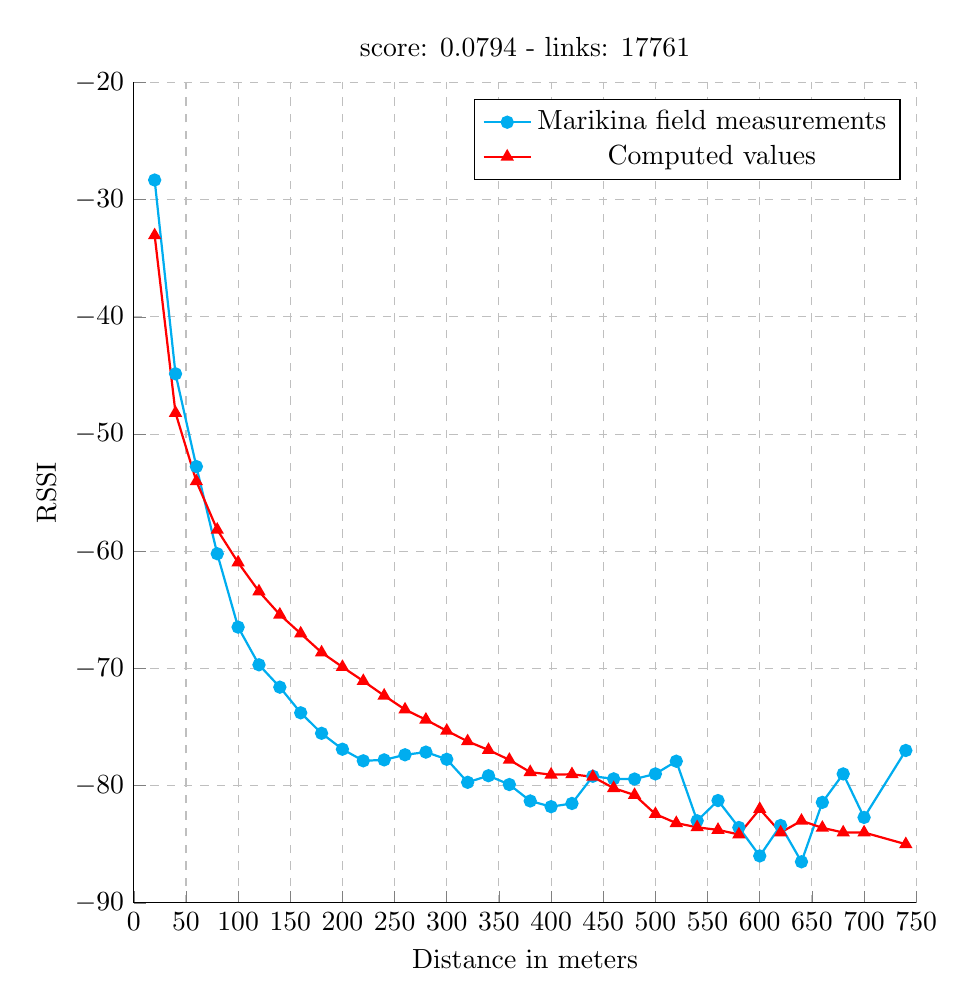
\begin{tikzpicture}
        \begin{axis}[
                title=score: 0.0794 - links: 17761,
                height=12cm, width=0.95\textwidth,
                ylabel={RSSI},
                xlabel={Distance in meters},
                axis lines*=left,
                xmin=0, xmax=750,
                enlargelimits=false,
                ymin=-90, ymax=-20,
                xtick={0, 50, 100, 150, 200, 250, 300, 350, 400, 450, 500, 550, 600, 650, 700, 750},
                ymajorgrids=true,
                xmajorgrids=true,
                grid style=dashed,
            ]

            \addplot[thick, solid, cyan, mark=*] coordinates {(20, -28.32345013477089) (40, -44.85830258302583) (60, -52.77323717948718) (80, -60.21201657458563) (100, -66.47435897435898) (120, -69.68905472636816) (140, -71.5976496922216) (160, -73.7866473149492) (180, -75.53428571428572) (200, -76.89289392378991) (220, -77.88135593220339) (240, -77.8035019455253) (260, -77.36784140969164) (280, -77.14030612244898) (300, -77.75299760191847) (320, -79.71686746987952) (340, -79.15481171548117) (360, -79.90728476821192) (380, -81.30909090909091) (400, -81.79746835443038) (420, -81.52272727272727) (440, -79.2) (460, -79.42105263157895) (480, -79.4375) (500, -79.0) (520, -77.91666666666667) (540, -83.0) (560, -81.27272727272727) (580, -83.57142857142857) (600, -86.0) (620, -83.4) (640, -86.5) (660, -81.42857142857143) (680, -79.0) (700, -82.71428571428571) (740, -77.0)};
            \addlegendentry{Marikina field measurements};

            \addplot[thick, solid, red, mark=triangle*] coordinates {(20,-33.04359925788497)(40,-48.19327731092437)(60,-54.03703703703704)(80,-58.16688567674113)(100,-60.96085858585859)(120,-63.43184421534937)(140,-65.41129831516353)(160,-67.02463054187191)(180,-68.64031007751937)(200,-69.87730061349693)(220,-71.07770961145194)(240,-72.32267441860465)(260,-73.50986842105263)(280,-74.37786259541984)(300,-75.32413793103449)(320,-76.22083333333333)(340,-76.95930232558139)(360,-77.8018018018018)(380,-78.84883720930233)(400,-79.06557377049181)(420,-79.03030303030303)(440,-79.25)(460,-80.21428571428571)(480,-80.8)(500,-82.42857142857143)(520,-83.2)(540,-83.55555555555556)(560,-83.77777777777777)(580,-84.16666666666667)(600,-82.0)(620,-84.0)(640,-83.0)(660,-83.6)(680,-84.0)(700,-84.0)(740,-85.0)};
            \addlegendentry{Computed values};
        \end{axis}
    \end{tikzpicture}
    \caption{Field measurements vs computed values}
    \label{plot:reachi-experiments:marikina-log-vs-computed}
\end{figure}


Finally a comparison of the computed results from \autoref{eq:pl} compared with the measurements from the Marikina log. Once again, links have been sorted into distance buckets and had the average \gls{rssi} for each bucket computed. The computed \gls{rssi}, was computed with \autoref{eq:pl} on the links from the Marikina log, but the field measured \gls{rssi} was removed. The computed \gls{rssi} was added instead, and the same sorting into distance buckets was done with the computed log. The result can be seen on \autoref{plot:reachi-experiments:marikina-log-vs-computed}. The computed score, once again, for a single link was 0.0794. \autoref{plot:reachi-experiments:marikina-log-vs-computed} shows that the function is off on the range from about 75 meters to 300 meters, however when compared with \autoref{plot:reachi-experiments:measurements-vs-ld} ours does indeed give a better result.